\documentclass[abstracton,12pt]{scrartcl}
    
\usepackage[utf8]{inputenc}
% \usepackage[T1]{fontenc}
\usepackage{fancyhdr}
\usepackage{graphicx}
\usepackage{tikz}
\usepackage{listings}
\usepackage{amssymb}
\usepackage{amsfonts}
\usepackage{amsmath}
\usepackage{amsthm}
\usepackage{pdfpages}
\usepackage{forest}
\usepackage{multicol}
\usepackage{varwidth}
\usepackage{verbatim}
%\usepackage{minted}
\usepackage{framed}
\usepackage[ruled,vlined]{algorithm2e}
\usepackage{caption}
\usepackage{subcaption}
\usepackage{cleveref}
\usepackage{soul}
% \usepackage{geometry}
% \usepackage{titlesec}

\forestset{qtree/.style={for tree={parent anchor=south, child anchor=north,align=left,inner sep=0pt}}}
\graphicspath{
  {images/},
  {images/1_unprod_nodes/},
  {images/2_unprod_nodes_tau/}
  {images/3_unprod_nodes_L/}
}

% \setlength{\multicolsep}{6.0pt plus 2.0pt minus 1.5pt}% 50% of original values
% \titleformat{\chapter}{}{\thechapter}{}{}
% \titlespacing{\chapter}{-100pt}{-100pt}{-100pt}

% --------- 

\titlehead{Department of Informatics, University of Zürich}
\subject{\vspace*{2cm}BSc Thesis}
\title{An Adaptive Index for Hierarchical Distributed Database Systems}
\author{
    Rafael Kallis\\[-5pt]
    \scriptsize Matrikelnummer: 14-708-887\\[-5pt]
    \scriptsize Email: \texttt{rk@rafaelkallis.com}
}
\date{\vspace*{2cm}February 1, 2018}
\publishers{
    \small supervised by Prof.\ Dr.\ Michael\ Böhlen and Kevin\ Wellenzohn \\[5cm]
    \begin{tikzpicture}[overlay]
    \node at (-3,-3) {
\includegraphics[height=1.5cm]{IFIlogo}};
    \node at (7,-3) {
\includegraphics[height=1.5cm]{dbtgBW}};
    \end{tikzpicture}
}

% \dedication{dedicated to xxx}

% --------- 

\theoremstyle{definition}

\newtheorem{definition}{Definition}
% \newtheorem{figure}{Figure}
\newtheorem{example}{Example}
% \newtheorem{theorem}{Theorem}
% \newtheorem{lemma}{Lemma}

\crefname{algocfline}{algorithm}{algorithms}
\Crefname{algocfline}{Algorithm}{Algorithms}

\crefname{figure}{Fig.}{Figs.}
\Crefname{figure}{Figure}{Figures}

\crefname{example}{Ex.}{Ex.}
\Crefname{example}{Example}{Examples}

% \newenvironment{proof}
%     {\noindent{\bf Proof:\rm}}{\hfill$\Box$\vspace{\medskipamount}}

\newenvironment{centerverbatim}{\par\centering\varwidth{\linewidth}\verbatim}
    {\endverbatim\endvarwidth\par}

% \def\bbbr{{\rm I\!R}}
% \def\bbbm{{\rm I\!M}}
% \def\bbbn{{\rm I\!N}}
% \def\bbbz{{\rm I\!Z}}

\definecolor{shadecolor}{rgb}{0.97,0.97,0.97}
    
\begin{document}

\maketitle

% \chapter*{Acknowledgements}

% \chapter*{Zusammenfassung}

\newpage

% \tableofcontents
\listoffigures
% \listoftables

\newpage

% \begin{abstract}
%   Frequently adding and removing data from hierarchical indexes causes them to
%   repeatedly grow and shrink. A single insertion or deletion can trigger a
%   sequence of structural index modifications (node insertions/deletions) in a
%   hierarchical index. Skewed and update-heavy workloads trigger repeated
%   structural index updates over a small subset of nodes to the index.

%   Informally, a frequently added or removed node is called \textit{volatile}.
%   Volatile nodes deteriorate index update performance due to two reasons.
%   First, frequent structural index modifications are expensive since they
%   cause many disk accesses. Second, frequent structural index modifications
%   also increase the likelihood of conflicting index updates by concurrent
%   transactions. Conflicting index updates further deteriorate update
%   performance since concurrency control protocols need to resolve the
%   conflict.


% \end{abstract}

\section{Introduction}

Frequently adding and removing data from hierarchical indexes causes them to
repeatedly grow and shrink. A single insertion or deletion can trigger a
sequence of structural index modifications (node insertions/deletions) in a
hierarchical index. Skewed and update-heavy workloads trigger repeated
structural index updates over a small subset of nodes to the index.

Informally, a frequently added or removed node is called \textit{volatile}.
Volatile nodes deteriorate index update performance due to two reasons. First,
frequent structural index modifications are expensive since they cause many disk
accesses. Second, frequent structural index modifications also increase the
likelihood of conflicting index updates by concurrent transactions. Conflicting
index updates further deteriorate update performance since concurrency control
protocols need to resolve the conflict.

Wellenzohn et al.~\cite{KW17} propose the Workload-Aware Property Index (WAPI).
The WAPI exploits the workloads' skewness by identifying and not removing
volatile nodes from the index, thus significantly reducing the number of
expensive structural index modifications. Since fewer nodes are
inserted/deleted, the likelihood of conflicting index updates by concurrent
transactions is reduced.

When the workload characteristics change, new index nodes can become volatile
while others cease to be volatile and become \textit{unproductive}. Unproductive
index nodes slow down queries as traversing an unproductive node is useless,
because neither the node itself nor any of its descendants contain an indexed
property and thus cannot yield a query match. Additionally, unproductive nodes
occupy storage space that could otherwise be reclaimed. lf the workload changes
frequently, unproductive nodes quickly accumulate in the index and the query
performance deteriorates over time. Therefore, unproductive nodes must be
cleaned up to keep query performance stable over time and reclaim disk space as
the workload changes.

Wellenzohn et al.~\cite{KW17} propose periodic Garbage Collection (GC), which
traverses the entire index subtree and prunes all unproductive index nodes at
once. Additionally we propose Query-Time Pruning (QTP), an incremental approach
to cleaning up unproductive nodes in the index. The idea is to turn queries into
updates. Since Oak already traverses unproductive nodes as part of query
processing, these nodes could be pruned at the same time. In comparison to GC,
with QTP only one query has to traverse an unproductive node, while subsequent
queries can skip this overhead and thus perform better.

The goal of this BSc thesis is to study, implement, and empirically compare GC
and QTP as proposed by \cite{KW17} in Apache Jackrabbit Oak (Oak).

% The goal of this project is to implement a WAPI, as proposed by \cite{KW17} in
% Apache Jackrabbit Oak (Oak) in order to improve the transactional throughput
% of Oak. In \Cref{sec:wapi} we describe how nodes are inserted, queried and
% deleted from the WAPI. Next, we describe how volatility is computed in
% \Cref{sec:volatility}. Finally, a reference implementation in Java is
% presented in \Cref{sec:implementation}.

\section{Background}

\subsection{Apache Jackrabbit Oak (Oak)}

% Oak\footnote{https://jackrabbit.apache.org/oak/} is a hierarchical distributed
% database system which makes use of a hierarchical index.
Oak is a hierarchical distributed database system which makes use of a
hierarchical index. Multiple transactions can work concurrently by making use of
Multiversion Concurrency Control (MVCC)~\cite{GW02}, a commonly used optimistic
concurrency control technique~\cite{TM11}.

\Cref{fig:architecture} depicts Oak's multi-tier architecture. Oak embodies the
\textit{Database Tier}.
% Whilst Oak is responsible for handling the database logic, it stores the
% actual data on MongoDB labeled as \textit{Persistence Tier}.
Whilst Oak is responsible for handling the database logic, it stores the actual
data on MongoDB\footnote{https://www.mongodb.com/what-is-mongodb}, labeled as
\textit{Persistence Tier}. On the other end, applications can make use of Oak as
shown in \Cref{fig:architecture} under \textit{Application Tier}.
% One such application is Adobe's enterprise content management system (CMS),
% the Adobe Experience Manager
w/One such application is Adobe's enterprise content management system (CMS),
the Adobe Experience
Manager\footnote{http://www.adobe.com/marketing-cloud/experience-manager.html}.

\begin{figure}[h]
  \begin{center}
    \begin{tikzpicture}[scale=0.7,thick]
	    \node (mongo) at (0, 0) {
\includegraphics[width = 0.7cm]{MONGO}}; \node
      (oak_a) at (-2, 2) {
\includegraphics[width = 0.7cm]{OAK}}; \node (oak_b)
      at (0, 2) {
\includegraphics[width = 0.7cm]{OAK}}; \node (oak_c) at (2, 2)
      {
\includegraphics[width = 0.7cm]{OAK}}; \node (app_a) at (-2, 4)
      {
\includegraphics[width = 0.7cm]{AEM}}; \node (app_b) at (0, 4)
      {
\includegraphics[width = 0.7cm]{AEM}}; \node (app_c) at (2, 4)
      {
\includegraphics[width = 0.7cm]{AEM}}; \node (mongo_desc) at (5, 0)
      {\footnotesize \textit{Persistence Tier}}; \node (oak_desc) at (5, 2)
      {\footnotesize \textit{Database Tier}}; \node (mongo_desc) at (5, 4)
      {\footnotesize \textit{Application Tier}}; \foreach \from/\to in
      {app_a/oak_a, app_b/oak_b, app_c/oak_c, oak_a/mongo, oak_b/mongo,
        oak_c/mongo} \draw [->] (\from) -- (\to);
    \end{tikzpicture}
  \end{center}
  % \vspace{-0.5cm}
  \caption{Apache Jackrabbit Oak's system architecture.}
  \label{fig:architecture}
\end{figure}

\subsection{Workload Aware Property Index (WAPI)}
\label{sec:wapi}

Oak mostly executes content-and-structure (CAS) queries~\cite{CM15}, defined as
follows.

\begin{definition}
  (CAS-Query): Given node $m$, property $k$ and value $v$, a CAS query
  $Q(k,v,m)$ returns all descendants of $m$ which have $k$ set to $v$, i.e
    $$ Q(k,v,m) = \{~n~|~n[k] = v \land n \in desc(m)~\}$$
  \end{definition}

  The WAPI is a hierarchical index and indexes the properties of nodes in order
  to answer CAS-queries efficiently. Additionally, it takes into account if an
  index node is volatile before performing structural index modifications. If a
  node is considered volatile, we do not remove it from the index.

  Volatility is the measure which is used by the WAPI in order to distinguish
  when to remove a node or not from the index.

  Wellenzohn et al.~\cite{KW17} propose to look at the recent transactional
  workload to check whether a node $n$ is volatile. The workload on Oak instance
  $O_i$ is represented by a sequence $H_i = \langle \ldots, G^a, G^b, G^c
  \rangle$ of snapshots, called a history. Let $t_n$ be the current time and
  $t(G^b)$ be the point in time snapshot $G^b$ was committed, $N(G^a)$ is the
  set of nodes which are members of snapshot $G^a$. $pre(G^b)$ is the
  predecessor of snapshot $G^b$ in $H_i$.

  Node $n$ is volatile iff $n$'s volatility count is at least $\tau$, called
  volatility threshold. The volatility count of $n$ is defined as the number of
  times $n$ was added or removed from snapshots in a sliding window of length
  $L$ over history $H_i$. Let $n^i$ denote version $i$ of node $n$ that belongs
  to the node set $N(G^i)$ of snapshot $G^i$. Given two snapshots $G^a$ and
  $G^b$ we write $n^a$ and $n^b$ to emphasize that nodes $n^a$ and $n^b$ are two
  versions of the same node $n$, i.e, they have the same absolute path from the
  root node.

\begin{definition}
  (Volatility Count): The volatility count $vol(n)$ of node $n$ is the number of
  times node $n$ was added or removed from snapshots contained in a sliding
  window with length $L$ over history $H_i$.
  \begin{align*}
    % \begin{split}
      vol(n) = | \{ G^b | G^b \in H_i \land t(G^b) \in [t_{n-L+1}, t_n] \land \exists G^a[ \\
      \qquad G^a = pre(G^b) \land ([n^a \notin N(G^a) \land n^b \in N(G^b)]\lor \\
      \qquad [n^a \in N(G^a) \land n^b \notin N(G^b)] )]\} |
    % \end{split}
  \end{align*}
  \label{def:vol_count}
\end{definition}

\begin{definition}
  (Volatile Node): Node $n$ is volatile iff $n$'s volatility count (see
  \Cref{def:vol_count}) is greater or equal than the volatility threshold
  $\tau$, i.e
  $$ volatile(n) \iff vol(n) \geq \tau $$
\end{definition}

\section{Unproductive Nodes}

When time passes and the database workload changes, volatile nodes cease to be
volatile and they become unproductive.
\begin{definition}
  (Unproductive Node): Node $n$ is unproductive iff $n$, and any descendant of
  $n$, is neither matching nor volatile, i.e
  $$ unproductive(n) \iff \nexists m (m \in (\{n\} \cup desc(n)) \land
  (volatile(m) \lor *m[k] \neq v)) $$
\end{definition}

\begin{example}
  Consider the snapshots depicted in \Cref{fig:unproductive_nodes}. Assume $H_h
  = \langle G^0,G^1,G^2,G^3,G^4,G^5,G^6 \rangle$. $O_h$ executes transactions
  $T_1, T_2, T_3, T_4, T_5, T_6$. Snapshot $G^0$ was committed at time $t(G^0) =
  t$. Given snapshot $G^0$, transaction $T_1$ adds property $x=1$
  \texttt{/a/b/d} and commits snapshot $G^1$ at time $t(G^1) = t + 1$. Next,
  transaction $T_2$ removes property $x$ from \texttt{/a/b/d} given snapshot
  $G^1$ and commits snapshot $G^2$ at time $t(G^2) = t + 2$. The index nodes are
  not pruned during $T^2$ since they are volatile. Transaction $T_3$ adds
  property $x=1$ to \texttt{/a/c/e} given $G^2$ and commits $G^3$ at time
  $t(G^3) = t+3$. Notice how \texttt{/i/x/1/a/b/d} and \texttt{/i/x/1/a/b} are
  the only unproductive index nodes and \texttt{/i/x/1/a/c/e} as well as
  \texttt{/i/x/1/a/c/e} are the only volatile index nodes in $G^3$. Transaction
  $T^4$ again adds property $x=1$ to \texttt{/a/b/d} given snapshot $G^3$ and
  commits snapshot $G^4$ at time $t(G^4) = t+4$. In $G^4$, nodes
  \texttt{/i/x/1/a/b/d} and \texttt{/i/x/1/a/b} are not unproductive anymore
  since \texttt{/i/x/1/a/b/d}'s content node is matching. Transaction $T^5$
  again removes property $x$ from \texttt{/a/b/d} given snapshot $G^4$ and
  commits snapshot $G^5$ at time $t(G^5) = t+5$. Since nodes
  \texttt{/i/x/1/a/b/d} and \texttt{/i/x/1/a/b} are not volatile, they are
  pruned from the property index during $T^5$. Finally transaction $T^6$ removes
  property $x=1$ from \texttt{/a/c/e} given snapshot $G^5$ and commits snapshot
  $G^6$ at time $t(G^6) = t+6$. Index nodes \texttt{/i/x/1/a/c/e} and
  \texttt{/i/x/1/a/c} are pruned from the property index during $T^6$ because
  they are not volatile.
\end{example}

\begin{figure}[h]
  \centering
  \begin{large}
  $$ G^0 \xrightarrow{\quad T_1 \quad} G^1 \xrightarrow{\quad T_2 \quad} G^2
  \xrightarrow{\quad T_3 \quad} G^3 \xrightarrow{\quad T_4 \quad} G^4
  \xrightarrow{\quad T_5 \quad} G^5 \xrightarrow{\quad T_6 \quad} G^6 $$
\end{large}
\begin{subfigure}{0.24\textwidth}
  \centering \scriptsize{
    \begin{framed}
      \begin{forest} qtree, [ [$\lambda:i$] [,phantom] [,phantom] [,phantom]
        [,phantom] [$\lambda:a$ [$\lambda:b$ [$\lambda:d$] ] [,phantom]
        [$\lambda:c$ [$\lambda:e$] ] ] ]
      \end{forest}

      \vspace{27mm}
    \end{framed}
  } \footnotesize{ Snapshot $G^0$
 
    $t(G^0) = t$ }
\end{subfigure}
\begin{subfigure}{0.24\textwidth}
  \centering \scriptsize{
    \begin{framed}
      \begin{forest} qtree, [ [$\lambda:i$ [$\lambda:x$ [$\lambda:1$
        [$\lambda:a$ [$\lambda:b$ [$\lambda:d$ \\ $x:1$] ] [,phantom] ] ] ] ]
        [,phantom] [,phantom] [,phantom] [,phantom] [$\lambda:a$ [$\lambda:b$
        [$\lambda:d$ \\ $x:1$] ] [,phantom] [$\lambda:c$ [$\lambda:e$] ] ] ]
      \end{forest}
    \end{framed}
  } \footnotesize{ Snapshot $G^1$
 
    $t(G^1) = t+1$ }
\end{subfigure}
\begin{subfigure}{0.24\textwidth}
  \centering \scriptsize{
    \begin{framed}
      \begin{forest} qtree, [ [$\lambda:i$ [$\lambda:x$ [$\lambda:1$
        [$\lambda:a$ [$\lambda:b$ [$\lambda:d$] ] [,phantom] ] ] ] ] [,phantom]
        [,phantom] [,phantom] [,phantom] [$\lambda:a$ [$\lambda:b$ [$\lambda:d$]
        ] [,phantom] [$\lambda:c$ [$\lambda:e$] ] ] ]
      \end{forest}

      \vspace{3.2mm}
    \end{framed}
  } \footnotesize{ Snapshot $G^2$
 
    $t(G^2) = t+2$ }
\end{subfigure}
\begin{subfigure}{0.24\textwidth}
  \centering \scriptsize{
    \begin{framed}
      \begin{forest} qtree, [ [$\lambda:i$ [$\lambda:x$ [$\lambda:1$
        [$\lambda:a$ [$\lambda:b$ [$\lambda:d$] ] [,phantom] [$\lambda:c$
        [$\lambda:e$ \\ $x:1$] ] ] ] ] ] [,phantom] [,phantom] [,phantom]
        [,phantom] [$\lambda:a$ [$\lambda:b$ [$\lambda:d$] ] [,phantom]
        [$\lambda:c$ [$\lambda:e$ \\ $x:1$] ] ] ]
      \end{forest}
    \end{framed}
  } \footnotesize{ Snapshot $G^3$
 
    $t(G^3) = t+3$ }
\end{subfigure}

\vspace{5mm}

\begin{subfigure}{0.24\textwidth}
  \centering \scriptsize{
    \begin{framed}
      \begin{forest} qtree, [ [$\lambda:i$ [$\lambda:x$ [$\lambda:1$
        [$\lambda:a$ [$\lambda:b$ [$\lambda:d$ \\ $x:1$] ] [,phantom]
        [$\lambda:c$ [$\lambda:e$ \\ $x:1$] ] ] ] ] ] [,phantom] [,phantom]
        [,phantom] [,phantom] [$\lambda:a$ [$\lambda:b$ [$\lambda:d$ \\ $x:1$] ]
        [,phantom] [$\lambda:c$ [$\lambda:e$ \\ $x:1$] ] ] ]
      \end{forest}
    \end{framed}
  } \footnotesize{ Snapshot $G^4$
 
    $t(G^4) = t+4$ }
\end{subfigure}
\begin{subfigure}{0.24\textwidth}
  \centering \scriptsize{
    \begin{framed}
      \begin{forest} qtree, [ [$\lambda:i$ [$\lambda:x$ [$\lambda:1$
        [$\lambda:a$ [,phantom] [,phantom] [$\lambda:c$ [$\lambda:e$ \\ $x:1$] ]
        ] ] ] ] [,phantom] [,phantom] [,phantom] [,phantom] [$\lambda:a$
        [$\lambda:b$ [$\lambda:d$] ] [,phantom] [$\lambda:c$ [$\lambda:e$ \\
        $x:1$] ] ] ]
      \end{forest}
    \end{framed}
  } \footnotesize{ Snapshot $G^5$
 
    $t(G^5) = t+5$ }
\end{subfigure}
\begin{subfigure}{0.24\textwidth}
  \centering \scriptsize{
    \begin{framed}
      \begin{forest} qtree, [ [$\lambda:i$] [,phantom] [,phantom] [,phantom]
        [,phantom] [$\lambda:a$ [$\lambda:b$ [$\lambda:d$] ] [,phantom]
        [$\lambda:c$ [$\lambda:e$] ] ] ]
      \end{forest}

      \vspace{27mm}
    \end{framed}
  } \footnotesize{ Snapshot $G^6$
 
    $t(G^6) = t+6$ }
\end{subfigure}
\caption{Unproductive Nodes}
\caption*{
  Nodes \texttt{/i/x/1/a/b/d} and \texttt{/i/x/1/a/b} are unproductive in snapshot
  $G^3$. They are not volatile and don't match either.
}
\label{fig:unproductive_nodes}
\end{figure}

Unproductive nodes slow down queries. During query execution, traversing an
unproductive node is useless, because neither the node itself nor any of its
descendants contains an indexed property and therefore cannot contribute a query
match. We formalize the statements above into the following scientific
questions:

\begin{shaded}
  \begin{itemize}
  \item[$Q_1$:] Query execution runtime increases over time.
  \item[$Q_2$:] Unproductive nodes account for the increase in query execution
    runtime.
  \end{itemize}
\end{shaded}

We recorded the query execution runtime throughout the experiment and present
the data below.
\Cref{fig:query_runtime_synthetic_millis,fig:query_runtime_aem_millis} show the
recorded query runtime over time as observed from the synthetic and AEM dataset respectively. 
\Cref{fig:query_runtime_synthetic_updates,fig:query_runtime_aem_updates} show the
recorded query runtime over update operations from the synthetic and AEM dataset respectively. 

\begin{figure}[h]
  \centering
  \begin{subfigure}{0.49\linewidth}
    \centering
    Synthetic
  \end{subfigure}
  \begin{subfigure}{0.49\linewidth}
    \centering
    AEM
  \end{subfigure}
  \begin{subfigure}{0.49\linewidth}
    \centering
    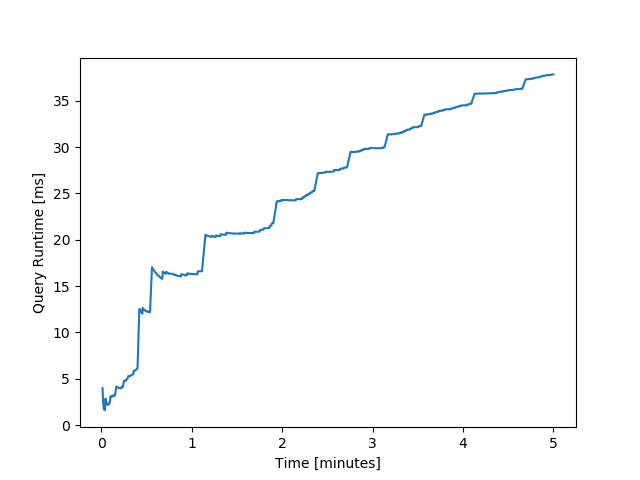
\includegraphics[width=8cm]{millis_query_runtime}
    \caption{}
    \label{fig:query_runtime_synthetic_millis}
  \end{subfigure}
  \begin{subfigure}{0.49\linewidth}
    \centering
    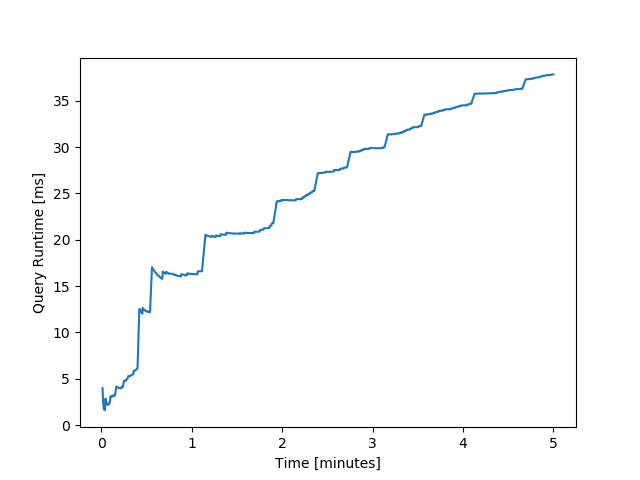
\includegraphics[width=8cm]{millis_query_runtime}
    \caption{}
    \label{fig:query_runtime_aem_millis}
  \end{subfigure}
  \begin{subfigure}{0.49\linewidth}
    \centering
    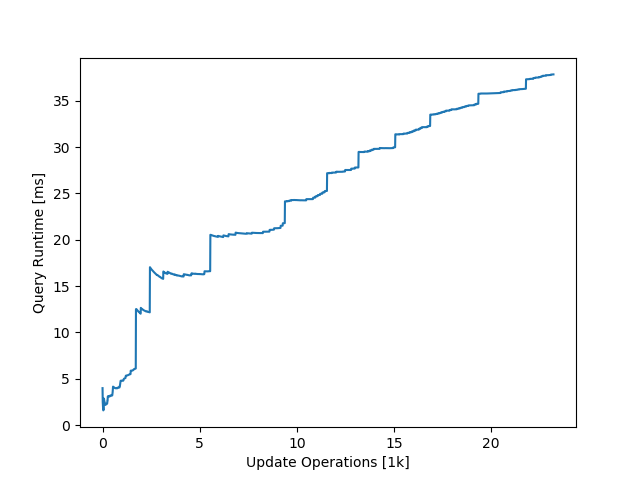
\includegraphics[width=8cm]{updates_query_runtime}
    \caption{}
    \label{fig:query_runtime_synthetic_updates}
  \end{subfigure}
  \begin{subfigure}{0.49\linewidth}
    \centering
    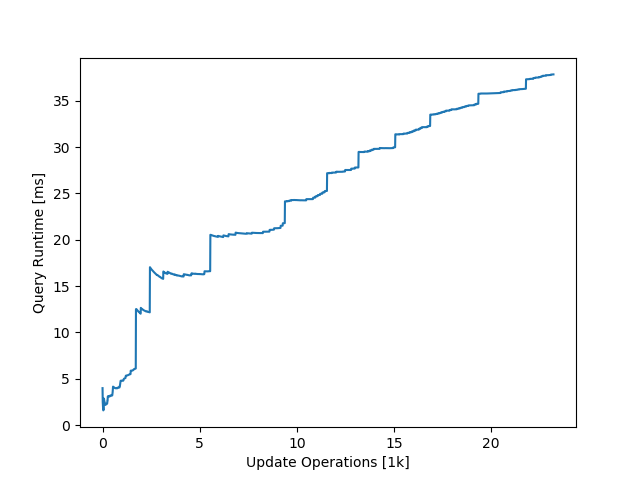
\includegraphics[width=8cm]{updates_query_runtime}
    \caption{}
    \label{fig:query_runtime_aem_updates}
  \end{subfigure}
  \caption{Query Execution Runtime}
  \label{fig:query_runtime}
\end{figure}

Next, we present data regarding the type of index nodes being traversed while
executing a query.
\Crefrange{fig:trav_nodes_synthetic_millis}{fig:trav_nodes_aem_updates} depict
the number of traversed volatile and unproductive index nodes during query
execution with respect to time and update operations from our datasets.
Additionally,
\Crefrange{fig:trav_node_density_synthetic_millis}{fig:trav_node_density_aem_updates}
show the density of volatile and unproductive nodes over time and update
operations from our datasets.

\begin{figure}[h]
  \centering
  \begin{subfigure}{0.49\linewidth}
    \centering
    Synthetic
  \end{subfigure}
  \begin{subfigure}{0.49\linewidth}
    \centering
    AEM
  \end{subfigure}
  \begin{subfigure}{0.49\linewidth}
    \centering
    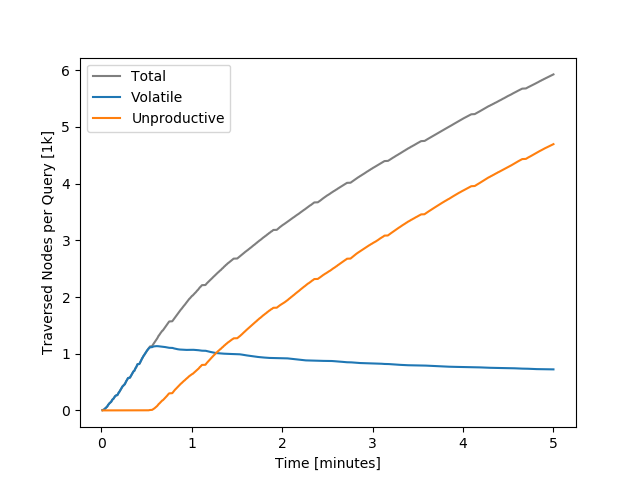
\includegraphics[width=7cm]{millis_traversed_index_nodes}
    \caption{}
    \label{fig:trav_nodes_synthetic_millis}
  \end{subfigure}
  \begin{subfigure}{0.49\linewidth}
    \centering
    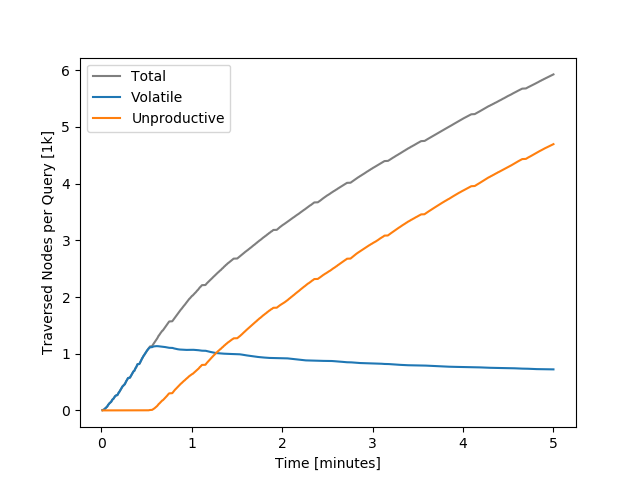
\includegraphics[width=7cm]{millis_traversed_index_nodes} 
    \caption{}
    \label{fig:trav_nodes_aem_millis}
  \end{subfigure}
  \begin{subfigure}{0.49\linewidth}
    \centering
    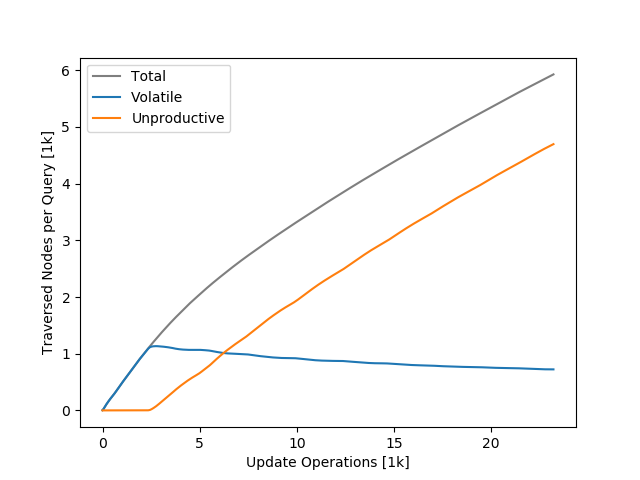
\includegraphics[width=7cm]{updates_traversed_index_nodes}
    \caption{}
    \label{fig:trav_nodes_synthetic_updates}
  \end{subfigure}
  \begin{subfigure}{0.49\linewidth}
    \centering
    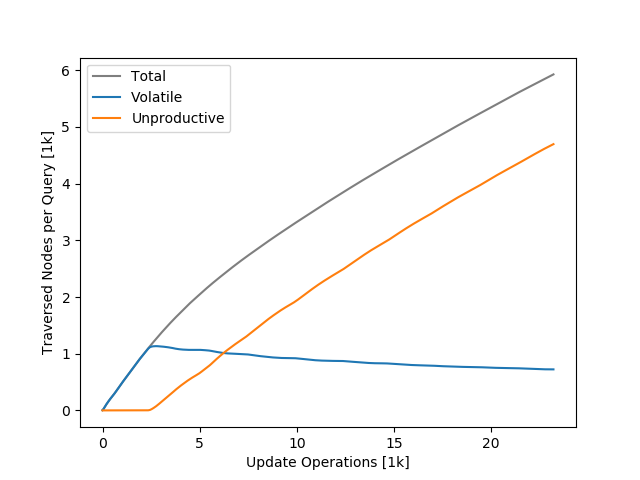
\includegraphics[width=7cm]{updates_traversed_index_nodes}
    \caption{}
    \label{fig:trav_nodes_aem_updates}
  \end{subfigure}

  % index density
  \begin{subfigure}{0.49\linewidth}
    \centering
    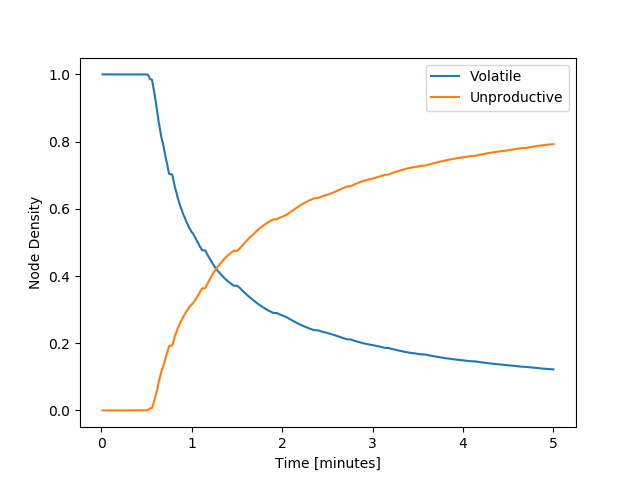
\includegraphics[width=7cm]{millis_index_node_density}
    \caption{}
    \label{fig:trav_node_density_synthetic_millis}
  \end{subfigure}
  \begin{subfigure}{0.49\linewidth}
    \centering
    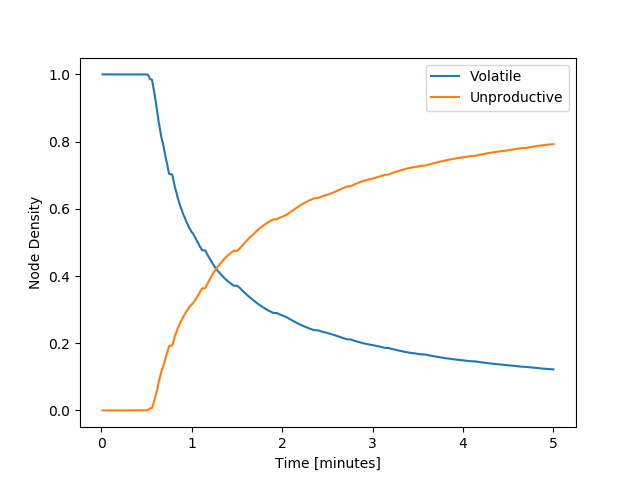
\includegraphics[width=7cm]{millis_index_node_density} 
    \caption{}
    \label{fig:trav_node_density_aem_millis}
  \end{subfigure}
  \begin{subfigure}{0.49\linewidth}
    \centering
    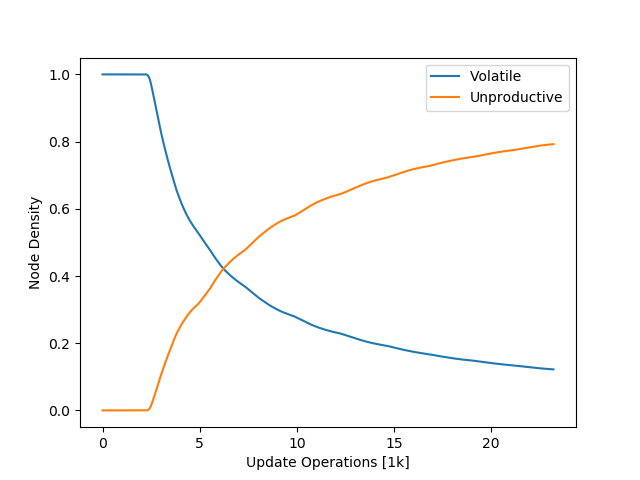
\includegraphics[width=7cm]{updates_index_node_density}
    \caption{}
    \label{fig:trav_node_density_synthetic_updates}
  \end{subfigure}
  \begin{subfigure}{0.49\linewidth}
    \centering
    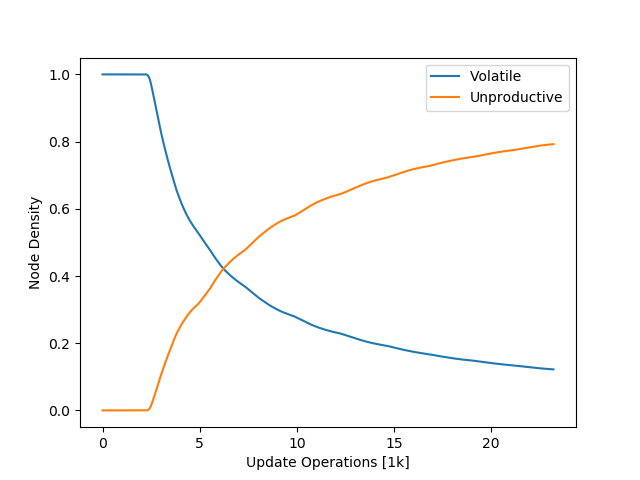
\includegraphics[width=7cm]{updates_index_node_density}
    \caption{}
    \label{fig:trav_node_density_aem_updates}
  \end{subfigure}
 \caption{Index nodes encountered while executing a query}
 \label{fig:query_runtime}
\end{figure}

The collected data shows a significant increase in query execution runtime over the
recorded time. The number of unproductive nodes grows over time while the number
of volatile nodes seem to stall after 30 seconds. We also observe that the
majority of traversed nodes during query execution are unproductivea and
therefore must likely account for the increase in query runtime. Interestingly,
we also observe the volatile and unproductive node density to converge below
$0.2$ and above $0.8$ respectively.

\subsection{Volatility Threshold ($\tau$)}

Volatility threshold $\tau$ determines after how many insertions/deletions of an index node
it becomes volatile \cite{KW17}. In this section, we study the impact of
volatility threshold $\tau$ on unproductive nodes and query execution runtime.

We hypothesize that an increase in $\tau$ yields a decrease to the query
execution runtime.
An increase in $\tau$ yields a decrease to the number of traversed unproductive
nodes during query execution.
An increase in $\tau$ yields a decrease to the unproductive node density during
query execution.
A node is less likely to become volatile with higher values
of $\tau$ and thus less likely to become volatile. 
Less unproductive nodes cause lower query  runtimes since less nodes traversals
are required during query execution.

\begin{shaded}
  \begin{itemize}
  \item[$Q_3$:] An increase in $\tau$ yields a decrease to the query execution runtime. 
  \item[$Q_4$:] An increase in $\tau$ yields a decrease to the number of
    traversed unproductive nodes during query execution.
  \item[$Q_5$:] An increase in $\tau$ yields a decrease to the unproductive node
    density during query execution 
    runtime.
  \end{itemize}
\end{shaded}

\begin{figure}[h]
  \centering
  \begin{subfigure}{0.49\linewidth}
    \centering
    Synthetic
  \end{subfigure}
  \begin{subfigure}{0.49\linewidth}
    \centering
    AEM
  \end{subfigure}
  \begin{subfigure}{0.49\linewidth}
    \centering
    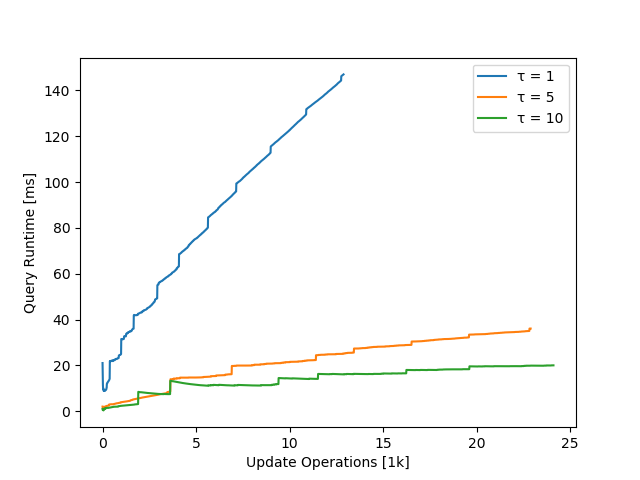
\includegraphics[width=8cm]{query_runtime_taus}
    \caption{}
    \label{fig:query_runtime_taus_synthetic}
  \end{subfigure}
  \begin{subfigure}{0.49\linewidth}
    \centering
    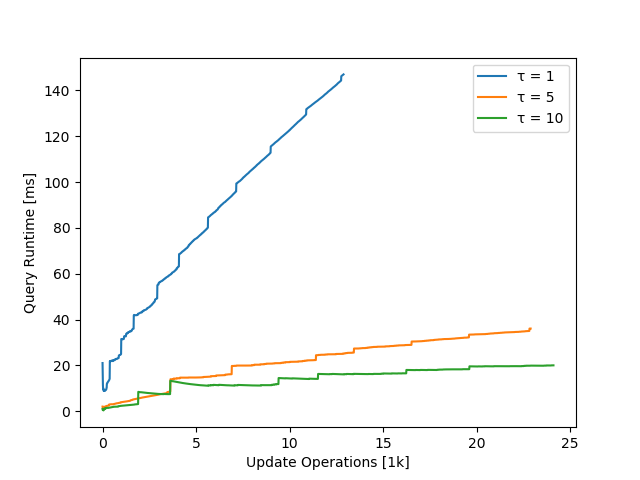
\includegraphics[width=8cm]{query_runtime_taus}
    \caption{}
    \label{fig:query_runtime_taus_aem}
  \end{subfigure}
  \begin{subfigure}{0.49\linewidth}
    \centering
    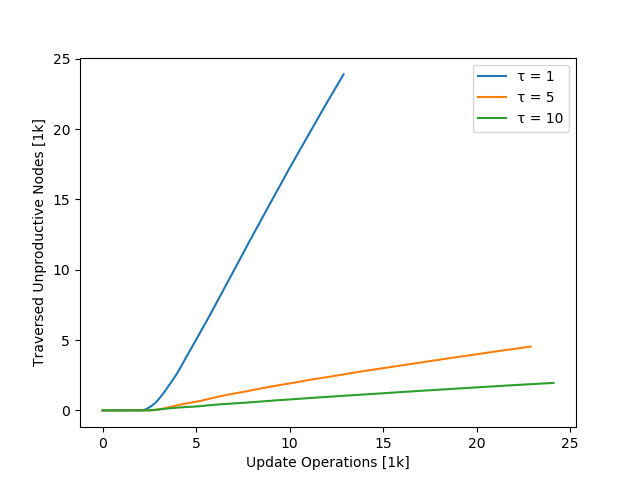
\includegraphics[width=8cm]{traversed_unprod_nodes_taus}
    \caption{}
    \label{fig:trav_unprod_nodes_taus_synthetic}
  \end{subfigure}
  \begin{subfigure}{0.49\linewidth}
    \centering
    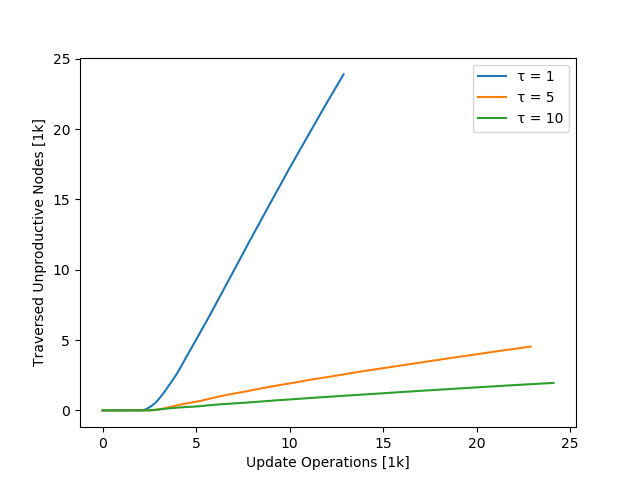
\includegraphics[width=8cm]{traversed_unprod_nodes_taus}
    \caption{}
    \label{fig:trav_unprod_nodes_taus_aem}
  \end{subfigure}
  \begin{subfigure}{0.49\linewidth}
    \centering
    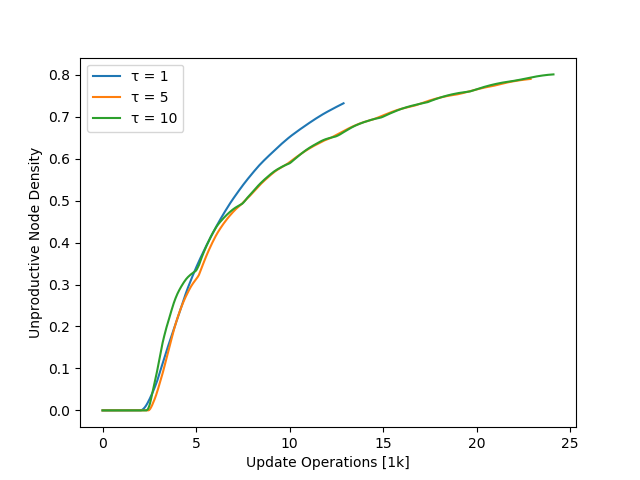
\includegraphics[width=8cm]{unprod_node_density_taus}
    \caption{}
    \label{fig:unprod_node_density_taus_synthetic}
  \end{subfigure}
  \begin{subfigure}{0.49\linewidth}
    \centering
    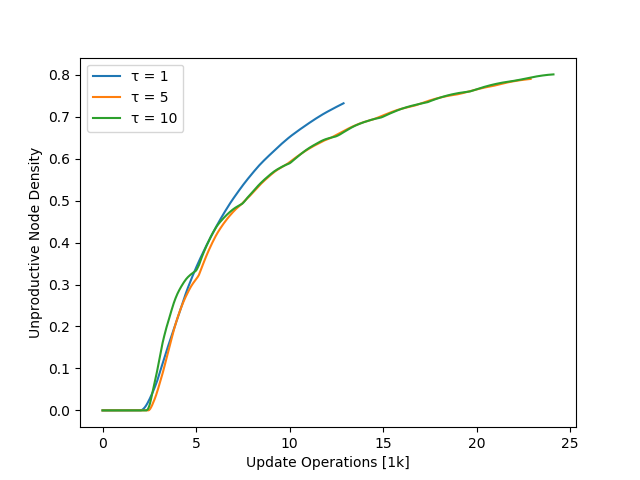
\includegraphics[width=8cm]{unprod_node_density_taus}
    \caption{}
    \label{fig:unprod_node_density_taus_aem}
  \end{subfigure}
  \caption{Impact of Volatility Threshold $\tau$}
\end{figure}

\begin{figure}[h]\ContinuedFloat
  \centering
  \begin{subfigure}{0.49\linewidth}
    \centering
    Synthetic
  \end{subfigure}
  \begin{subfigure}{0.49\linewidth}
    \centering
    AEM
  \end{subfigure}
  \begin{subfigure}{0.49\linewidth}
    \centering
    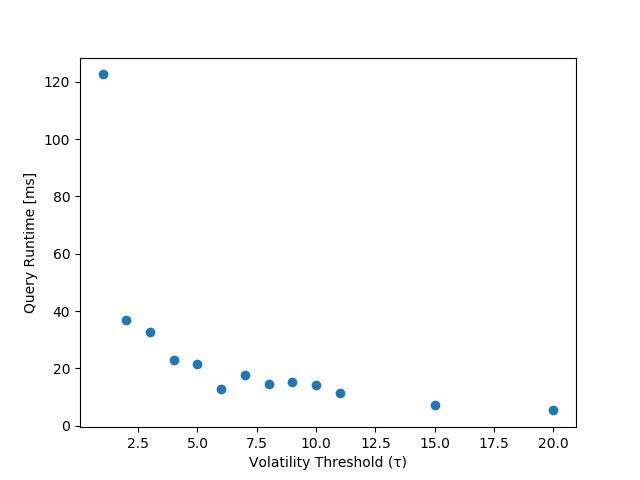
\includegraphics[width=8cm]{tau_query_runtime}
    \caption{}
    \label{fig:tau_query_runtime_synthetic}
  \end{subfigure}
  \begin{subfigure}{0.49\linewidth}
    \centering
    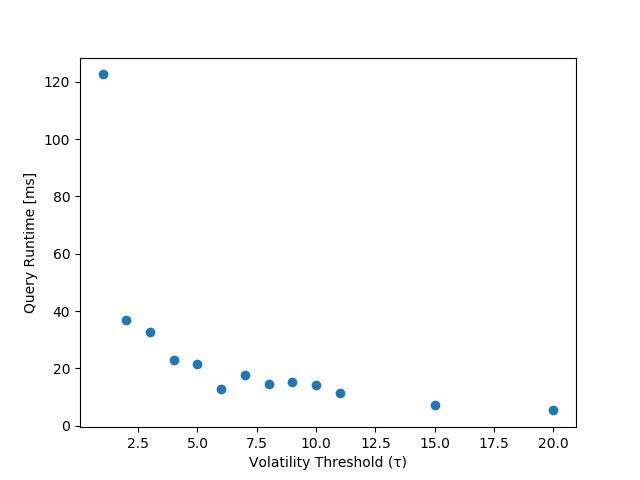
\includegraphics[width=8cm]{tau_query_runtime}
    \caption{}
    \label{fig:tau_query_runtime_aem}
  \end{subfigure}
  \begin{subfigure}{0.49\linewidth}
    \centering
    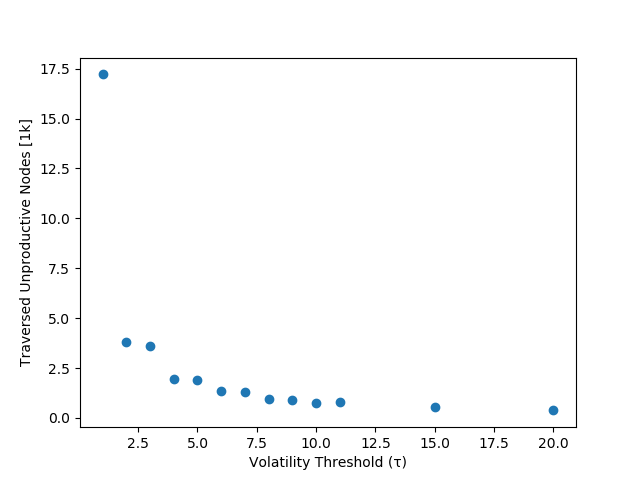
\includegraphics[width=8cm]{tau_unprod_nodes}
    \caption{}
    \label{fig:tau_unprod_nodes_synthetic}
  \end{subfigure}
  \begin{subfigure}{0.49\linewidth}
    \centering
    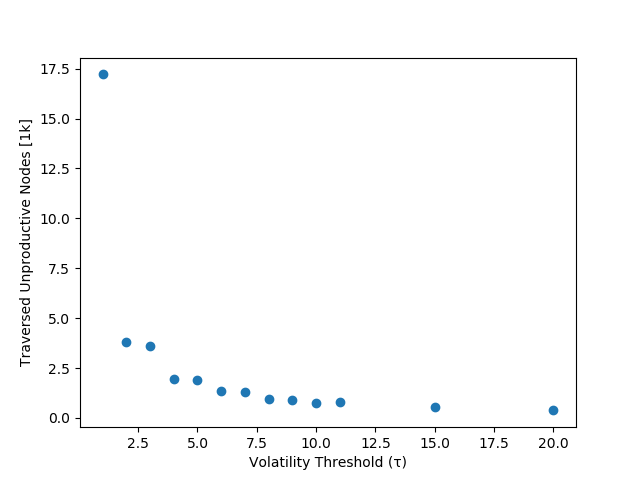
\includegraphics[width=8cm]{tau_unprod_nodes}
    \caption{}
    \label{fig:tau_unprod_nodes_aem}
  \end{subfigure}
  \begin{subfigure}{0.49\linewidth}
    \centering
    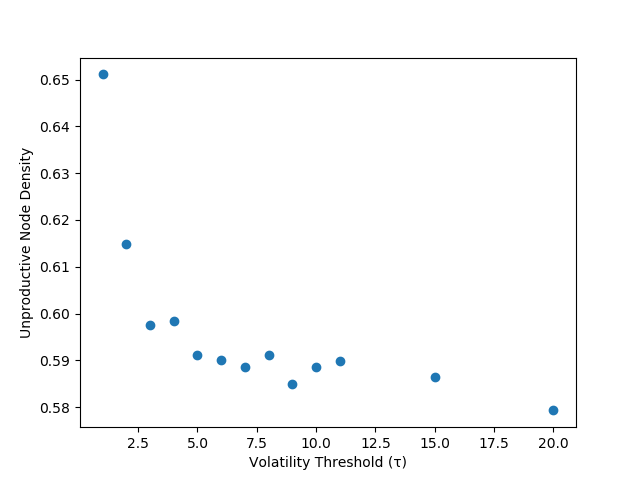
\includegraphics[width=8cm]{tau_unprod_node_density}
    \caption{}
    \label{fig:tau_unprod_node_density_synthetic}
  \end{subfigure}
  \begin{subfigure}{0.49\linewidth}
    \centering
    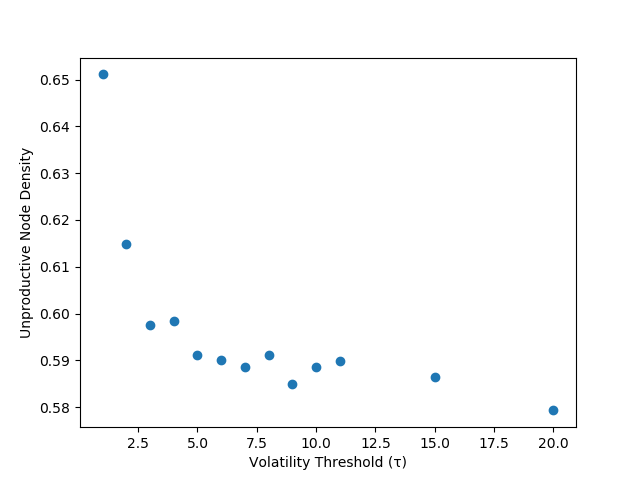
\includegraphics[width=8cm]{tau_unprod_node_density}
    \caption{}
    \label{fig:tau_unprod_node_density_aem}
  \end{subfigure}
  \caption{Impact of Volatility Threshold $\tau$ (cont.)}
  \label{fig:volatility_threshold}
\end{figure}

\subsection{Sliding window Length ($L$)}

\begin{figure}[h]
  \centering
  \begin{subfigure}{0.49\linewidth}
    \centering
    Synthetic
  \end{subfigure}
  \begin{subfigure}{0.49\linewidth}
    \centering
    AEM
  \end{subfigure}
  \begin{subfigure}{0.49\linewidth}
    \centering
    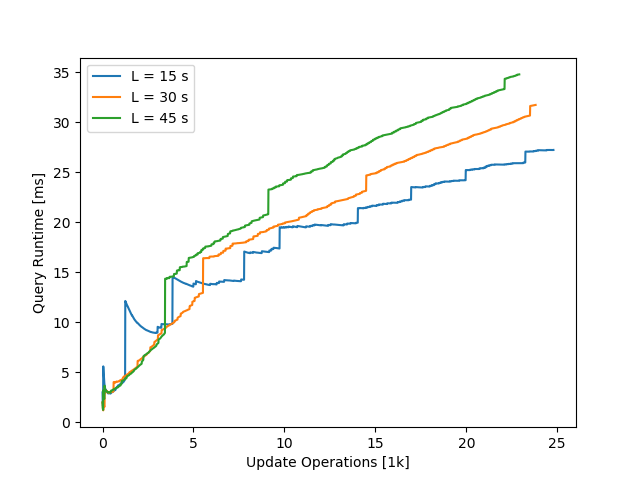
\includegraphics[width=8cm]{query_runtime_Ls}
    \caption{}
    \label{fig:query_runtime_Ls_synthetic}
  \end{subfigure}
  \begin{subfigure}{0.49\linewidth}
    \centering
    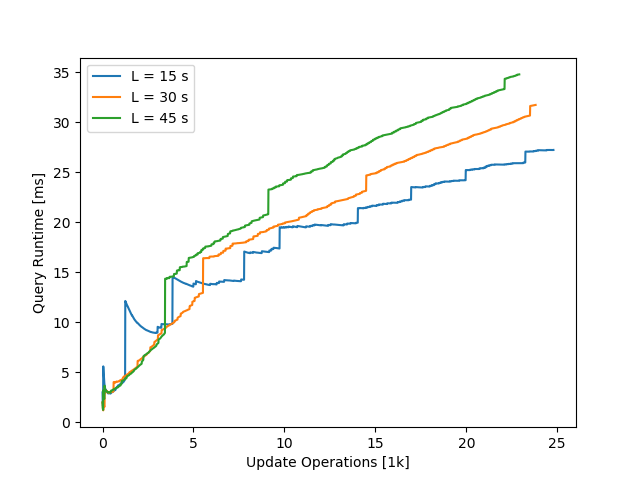
\includegraphics[width=8cm]{query_runtime_Ls}
    \caption{}
    \label{fig:query_runtime_Ls_aem}
  \end{subfigure}
  \begin{subfigure}{0.49\linewidth}
    \centering
    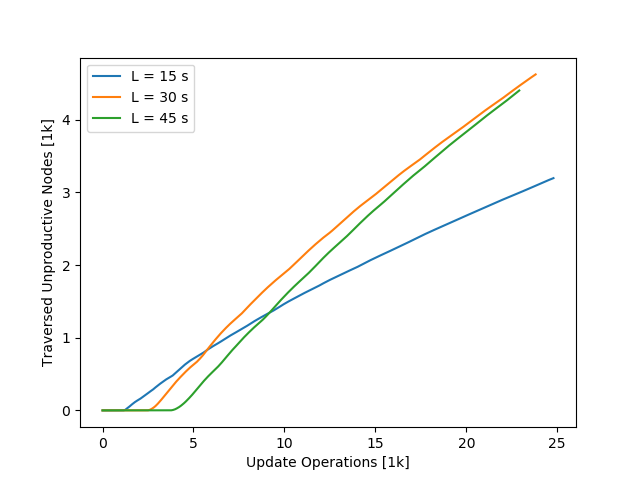
\includegraphics[width=8cm]{traversed_unprod_nodes_Ls}
    \caption{}
    \label{fig:trav_unprod_nodes_Ls_synthetic}
  \end{subfigure}
  \begin{subfigure}{0.49\linewidth}
    \centering
    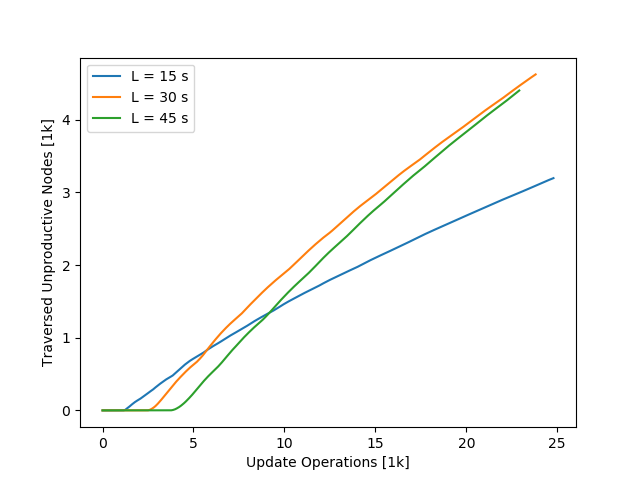
\includegraphics[width=8cm]{traversed_unprod_nodes_Ls}
    \caption{}
    \label{fig:trav_unprod_nodes_Ls_aem}
  \end{subfigure}
  \begin{subfigure}{0.49\linewidth}
    \centering
    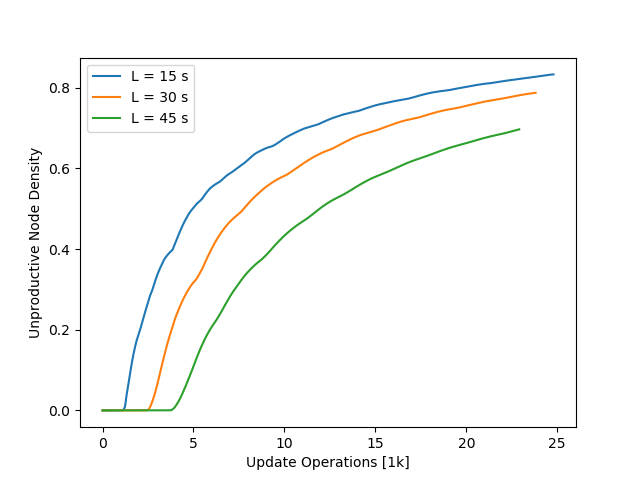
\includegraphics[width=8cm]{unprod_node_density_Ls}
    \caption{}
    \label{fig:unprod_node_density_Ls_synthetic}
  \end{subfigure}
  \begin{subfigure}{0.49\linewidth}
    \centering
    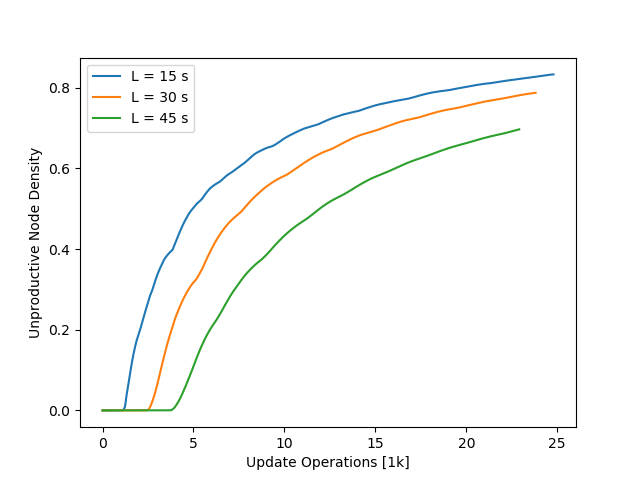
\includegraphics[width=8cm]{unprod_node_density_Ls}
    \caption{}
    \label{fig:unprod_node_density_Ls_aem}
  \end{subfigure}
  \caption{Impact of Sliding Window Length $L$}
\end{figure}

\begin{figure}[h]\ContinuedFloat
  \centering
  \begin{subfigure}{0.49\linewidth}
    \centering
    Synthetic
  \end{subfigure}
  \begin{subfigure}{0.49\linewidth}
    \centering
    AEM
  \end{subfigure}
  \begin{subfigure}{0.49\linewidth}
    \centering
    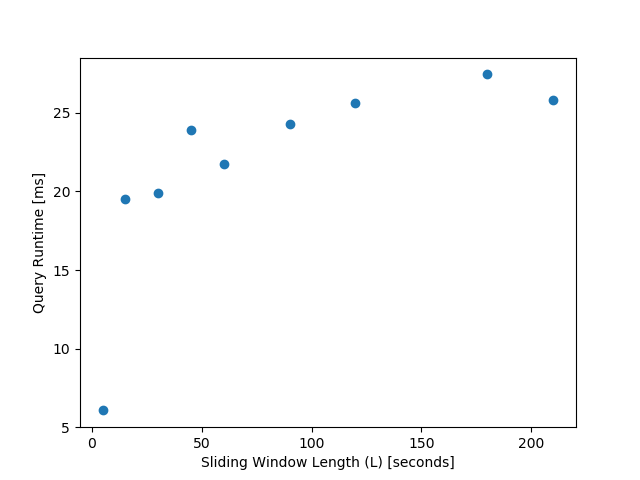
\includegraphics[width=8cm]{L_query_runtime}
    \caption{}
    \label{fig:L_query_runtime_synthetic}
  \end{subfigure}
  \begin{subfigure}{0.49\linewidth}
    \centering
    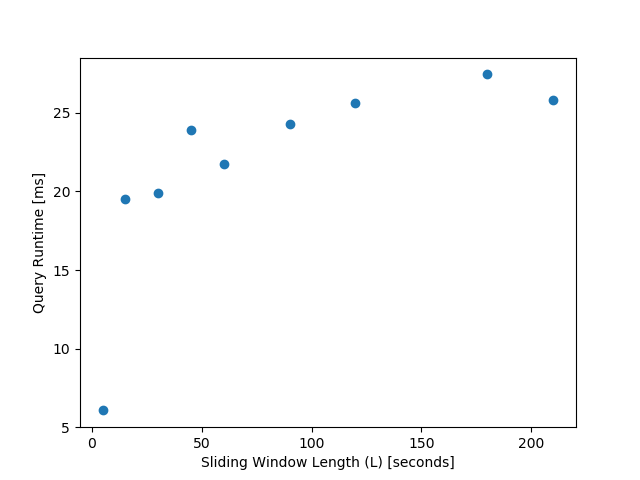
\includegraphics[width=8cm]{L_query_runtime}
    \caption{}
    \label{fig:L_query_runtime_aem}
  \end{subfigure}
  \begin{subfigure}{0.49\linewidth}
    \centering
    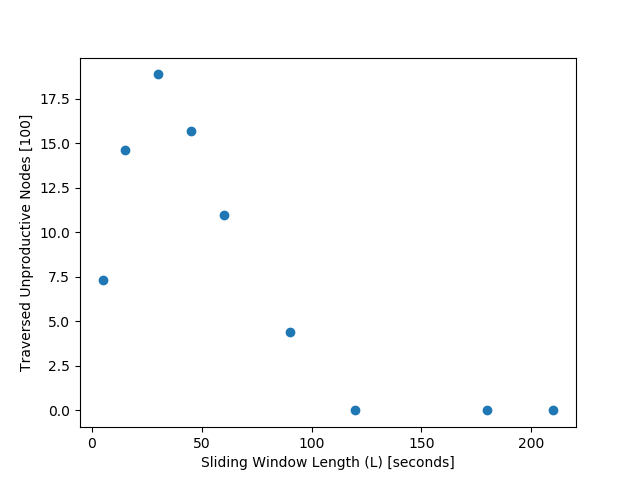
\includegraphics[width=8cm]{L_unprod_nodes}
    \caption{}
    \label{fig:L_unprod_nodes_synthetic}
  \end{subfigure}
  \begin{subfigure}{0.49\linewidth}
    \centering
    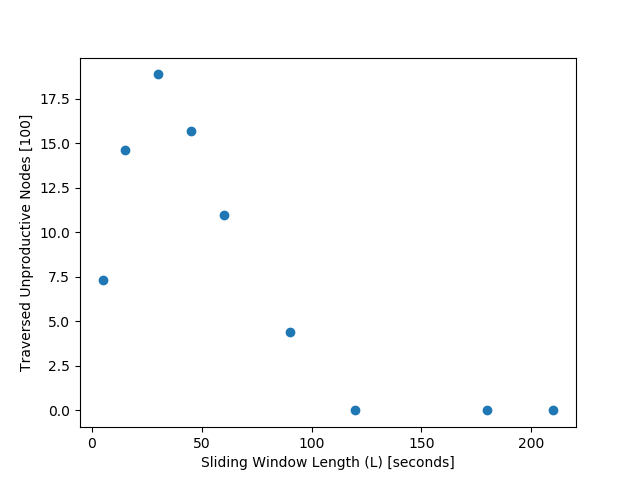
\includegraphics[width=8cm]{L_unprod_nodes}
    \caption{}
    \label{fig:L_unprod_nodes_aem}
  \end{subfigure}
  \begin{subfigure}{0.49\linewidth}
    \centering
    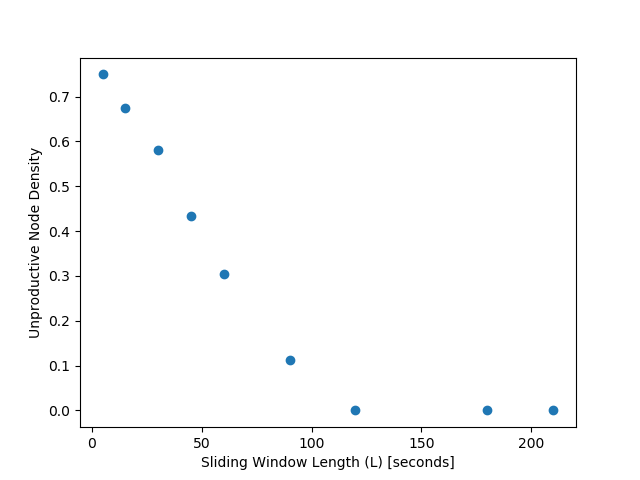
\includegraphics[width=8cm]{L_unprod_node_density}
    \caption{}
    \label{fig:L_unprod_node_density_synthetic}
  \end{subfigure}
  \begin{subfigure}{0.49\linewidth}
    \centering
    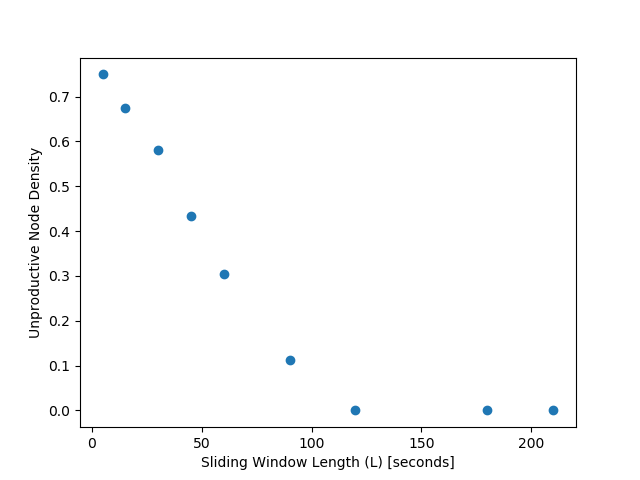
\includegraphics[width=8cm]{L_unprod_node_density}
    \caption{}
    \label{fig:L_unprod_node_density_aem}
  \end{subfigure}
  \caption{Impact of Sliding Window length $L$ (cont.)}
  \label{fig:sliding_window_length}
\end{figure}


% \tau / unproductive nodes

% L / unproductive nodes

\section{Periodic Garbage Collection (GC)}

\section{Query Time Pruning (QTP)}

\section{Experimental Evaluation}

% In order to empirically evaluate and compare GC and QTP under a changing
% workload, a experiment harness has to be setup.

% datasets

% zipf distribution

% changing Workload

% parameters

\newpage

\bibliographystyle{abbrv}
\bibliography{thesis}

\end{document}
